\chapter{Графики}
\label{ch:plot}

Краткое описанике по построению графиков при помощи PGFPlots \cite{habrpgfplots}.

	\begin{figure}[ht]
        \centering
		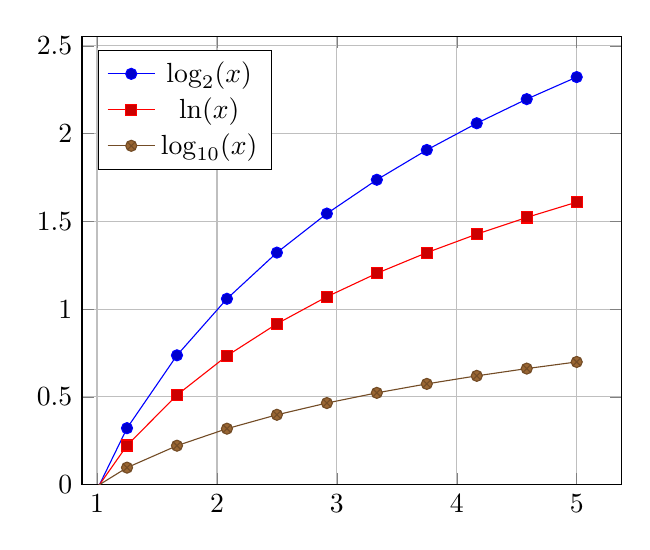
\begin{tikzpicture}
			\begin{axis} [
				legend pos = north west, 
				ymin = 0, 
				grid = major
			]
			\legend{ 
				$\log_2(x)$, 
				$\ln(x)$, 
				$\log_{10}(x)$
			};
			\addplot {log2(x)};
			\addplot {ln(x)};
			\addplot {log10(x)};
			\end{axis}
		\end{tikzpicture}
		\caption{Простая подпись к графикам}\label{}
	\end{figure}

А здесь будет продолжение текста.
\endinput